\section{\stmt{UND}  Funktion}

$$ \text{\stmt{UND( \syntax{Bedingung\_1}; \syntax{Bedingung\_2}; \ldots; \syntax{Bedingung\_255})}} $$

Die \stmt{UND} Funktion gibt WAHR zurück, wenn alle Bedingungen WAHR sind.

\begin{description}[labelindent=0cm, leftmargin=3cm, font=\mdseries, labelwidth=3cm,style=nextline]
\item[Beispiele] \stmt{=UND( 1>2 ; 2<3 )} $\Rightarrow$ FALSCH\\
\stmt{=UND( 1>0 ; 8/4=2 )} $\Rightarrow$ WAHR
\end{description}
%
Die \stmt{UND} Funktion kommt sehr häufig in Formeln mit einer \stmt{WENN} Bedingung vor.
%
	\begin{figure}[H]
		\centering
			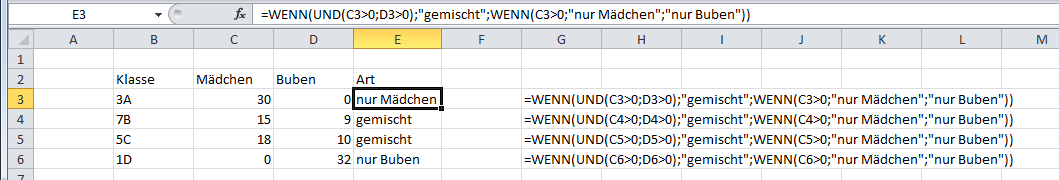
\includegraphics[width=16cm]{images/und_mit_wenn_b}
%			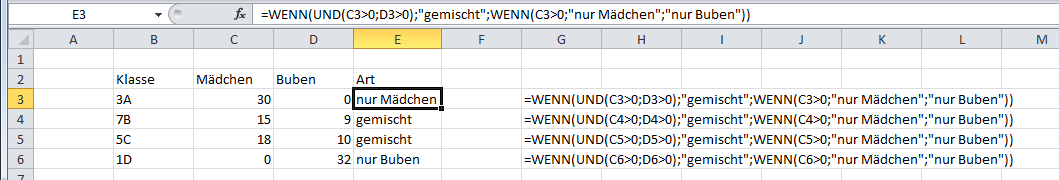
\includegraphics[scale=0.7]{images/und_mit_wenn_b}
		\caption{\stmt{WENN} und \stmt{UND} in einer Formel}
		\label{fig:wenn_mit_und}
	\end{figure}
